\documentclass[journal]{vgtc}               % final (journal style)
%\documentclass[review,journal]{vgtc}         % review (journal style)
%\documentclass[widereview]{vgtc}             % wide-spaced review
%\documentclass[preprint,journal]{vgtc}       % preprint (journal style)

%% Uncomment one of the lines above depending on where your paper is
%% in the conference process. ``review'' and ``widereview'' are for review
%% submission, ``preprint'' is for pre-publication, and the final version
%% doesn't use a specific qualifier.

%% Please use one of the ``review'' options in combination with the
%% assigned online id (see below) ONLY if your paper uses a double blind
%% review process. Some conferences, like IEEE Vis and InfoVis, have NOT
%% in the past.

%% Please note that the use of figures other than the optional teaser is not permitted on the first page
%% of the journal version.  Figures should begin on the second page and be
%% in CMYK or Grey scale format, otherwise, colour shifting may occur
%% during the printing process.  Papers submitted with figures other than the optional teaser on the
%% first page will be refused. Also, the teaser figure should only have the
%% width of the abstract as the template enforces it.

%% These few lines make a distinction between latex and pdflatex calls and they
%% bring in essential packages for graphics and font handling.
%% Note that due to the \DeclareGraphicsExtensions{} call it is no longer necessary
%% to provide the the path and extension of a graphics file:
%% 
\includegraphics{diamondrule} is completely sufficient.
%%
\ifpdf%                                % if we use pdflatex
  \pdfoutput=1\relax                   % create PDFs from pdfLaTeX
  \pdfcompresslevel=9                  % PDF Compression
  \pdfoptionpdfminorversion=7          % create PDF 1.7
  \ExecuteOptions{pdftex}
  \usepackage{graphicx}                % allow us to embed graphics files
  \DeclareGraphicsExtensions{.pdf,.png,.jpg,.jpeg} % for pdflatex we expect .pdf, .png, or .jpg files
\else%                                 % else we use pure latex
  \ExecuteOptions{dvips}
  \usepackage{graphicx}                % allow us to embed graphics files
  \DeclareGraphicsExtensions{.eps}     % for pure latex we expect eps files
\fi%

%% it is recomended to use ``\autoref{sec:bla}'' instead of ``Fig.~\ref{sec:bla}''
\graphicspath{{figures/}{pictures/}{images/}{./}} % where to search for the images

\usepackage{microtype}                 % use micro-typography (slightly more compact, better to read)
\PassOptionsToPackage{warn}{textcomp}  % to address font issues with \textrightarrow
\usepackage{textcomp}                  % use better special symbols
\usepackage{mathptmx}                  % use matching math font
\usepackage{times}                     % we use Times as the main font
\renewcommand*\ttdefault{txtt}         % a nicer typewriter font
\usepackage{cite}                      % needed to automatically sort the references
\usepackage{tabu}                      % only used for the table example
\usepackage{booktabs}                  % only used for the table example
%% We encourage the use of mathptmx for consistent usage of times font
%% throughout the proceedings. However, if you encounter conflicts
%% with other math-related packages, you may want to disable it.

%% In preprint mode you may define your own headline.
%\preprinttext{To appear in IEEE Transactions on Visualization and Computer Graphics.}

%% If you are submitting a paper to a conference for review with a double
%% blind reviewing process, please replace the value ``0'' below with your
%% OnlineID. Otherwise, you may safely leave it at ``0''.
\onlineid{0}

%% declare the category of your paper, only shown in review mode
\vgtccategory{Research}
%% please declare the paper type of your paper to help reviewers, only shown in review mode
%% choices:
%% * algorithm/technique
%% * application/design study
%% * evaluation
%% * system
%% * theory/model
\vgtcpapertype{please specify}

%% Paper title.
\title{Determining signal processing strategies to eliminate Flame Detector analogue noise generated by GHz frequency interference}

%% This is how authors are specified in the journal style

%% indicate IEEE Member or Student Member in form indicated below
\author{Daniel Sikar - Jupyter Notebook link https://smcse.city.ac.uk/student/aczd097/inm430.html}
\authorfooter{
%% insert punctuation at end of each item
\item
 Daniel Sikar MSc Data Science part-time student at City University of London. E-mail: daniel.sikar@city.ac.uk
}

%%%%%%%%%%%%%%%%%%%%%%%%%%%%%%%%%%%%%%%%%%%%%%%%%%%%%%%%%%%%%%%%
%%%%%%%%%%%%%%%%%%%%%%%%%% ABSTRACT %%%%%%%%%%%%%%%%%%%%%%%%%%%%
%%%%%%%%%%%%%%%%%%%%%%%%%%%%%%%%%%%%%%%%%%%%%%%%%%%%%%%%%%%%%%%%

%% \input{INM430-final-report-0.5-abstract.tex}

%%%%%%%%%%%%%%%%%%%%%%%%%%%%%%%%%%%%%%%%%%%%%%%%%%%%%%%%%%%%%%%%
%%%%%%%%%%%%%%%%%%%%%%%%%% KEYWORDS %%%%%%%%%%%%%%%%%%%%%%%%%%%%
%%%%%%%%%%%%%%%%%%%%%%%%%%%%%%%%%%%%%%%%%%%%%%%%%%%%%%%%%%%%%%%%

%% Keywords that describe your work. Will show as 'Index Terms' in journal
%% please capitalize first letter and insert punctuation after last keyword
\keywords{Signal processing, analogue noise, gigahertz frequency interference}

%% ACM Computing Classification System (CCS). 
%% See <http://www.acm.org/class/1998/> for details.
%% The ``\CCScat'' command takes four arguments.

\CCScatlist{ % not used in journal version
 \CCScat{K.6.1}{Management of Computing and Information Systems}%
{Project and People Management}{Life Cycle};
 \CCScat{K.7.m}{The Computing Profession}{Miscellaneous}{Ethics}
}

%% Uncomment below to include a teaser figure.
\teaser{
  \centering
  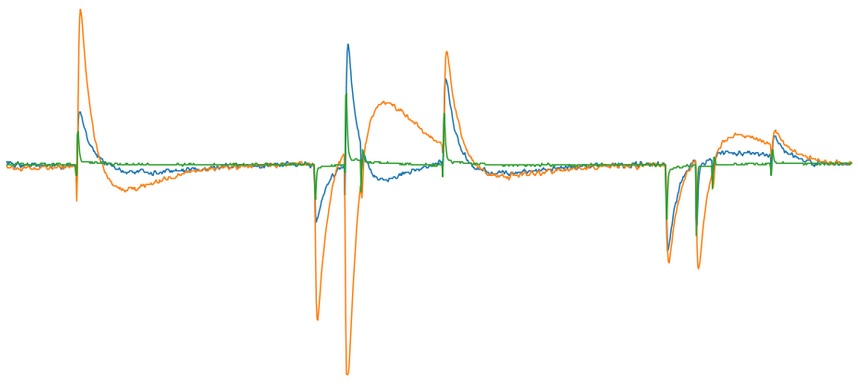
\includegraphics[width=\linewidth]{new-teaser.jpg}
  \caption{Analogue signals subject to radio frequency interference}
	\label{fig:teaser}
}

%% Uncomment below to disable the manuscript note
\renewcommand{\manuscriptnotetxt}{}

%% Copyright space is enabled by default as required by guidelines.
%% It is disabled by the 'review' option or via the following command:
% \nocopyrightspace

\vgtcinsertpkg

%%%%%%%%%%%%%%%%%%%%%%%%%%%%%%%%%%%%%%%%%%%%%%%%%%%%%%%%%%%%%%%%
%%%%%%%%%%%%%%%%%%%%%% START OF THE PAPER %%%%%%%%%%%%%%%%%%%%%%
%%%%%%%%%%%%%%%%%%%%%%%%%%%%%%%%%%%%%%%%%%%%%%%%%%%%%%%%%%%%%%%%%

\begin{document}

%% The ``\maketitle'' command must be the first command after the
%% ``\begin{document}'' command. It prepares and prints the title block.

%% the only exception to this rule is the \firstsection command

\firstsection{Introduction}

\maketitle

%%%%%%%%%%%%%%%%%%%%%%%%%%%%%%%%%%%%%%%%%%%%%%%%%%%%%%%%%%%%%%%%
%%%%%%%%%%%%%%%%%%%%%% INTRODUCTION %%%%%%%%%%%%%%%%%%%%%%%%%%%%
%%%%%%%%%%%%%%%%%%%%%%%%%%%%%%%%%%%%%%%%%%%%%%%%%%%%%%%%%%%%%%%%

%% INTRODUCTION


\subsection{Domain overview}
Flame detectors are widely used in areas subject to fire hazards such as oil and gas installations and chemical plants. Detectors consist of hardware and software subject to SIL (Security Integrity Level) certification, aiming and reducing risk effects. Standards such as the IEC 61508\cite{wiki:IEC61508} are used to certify equipment and ensure compliance.  

\subsection{Problems to be tackled}

To carry out the analysis the barriers to overcome consist of:

\begin{itemize}
\item processing log files
\item choosing appropriate libraries
\item engineer features to inform our decisions

\end{itemize}

\subsection{Analytical questions}

The analytical questions we want to ask is how can signal be differentiated from noise? Though distance functions? Linear regression? A combination of both?

\subsection{Objectives}

\begin{itemize}
\item Trial different techniques
\item Find a suitable model to eliminate noise (smoothing algorithm)

Note, this could be a combination of existing algorithms, to make best use of the attributes present in available dataset.
\end{itemize}

\subsection{Data source} 

The data being analysed consists of data logs generated by commercially available flame detectors. Twenty eight files were examined in total, generated under test conditions. One log file (Test45.log) containing real fire data, some of the remaining logs containing RF (radio frequency) data erroneously reported in software as fire - this will be shown in attributes.

The logs files were obtained from a flame detector undergoing Functional Safety of Electrical/Electronic/Programmable Electronic Safety-related Systems, as defined in the IEC 61508 standard \cite{wiki:IEC61508}. One log file (Test45.log) containing real fire data, the other logs, some containing RF (radio frequency) data erroneously reported in software as fire.

\subsection{Analysis strategy}

Once our signal and noise have been characterized, our analysis strategy consists of engineering features, as well as creating models to quantify the levels of noise and signal. Distance functions, fft transforms and filters, such as proposed by Savitzky and Golay \cite{Savitzky:1964} provide a scheme to smooth signals, eliminating noise. In this work, we shall examine such schemes and compare the end results, determining by sch observations a filtering strategy to eliminate noise generated by GHz frequency interference.


%%%%%%%%%%%%%%%%%%%%%%%%%%%%%%%%%%%%%%%%%%%%%%%%%%%%%%%%%%%%%%%%
%%%%%%%%%%%%%%%%% Findings and Reflections %%%%%%%%%%%%%%%%%%%%%
%%%%%%%%%%%%%%%%%%%%%%%%%%%%%%%%%%%%%%%%%%%%%%%%%%%%%%%%%%%%%%%%

\section{Discussion}

We processed our data by transforming hexadecimal encoded byte values into numerical valued between 0 and 255 (unsigned bytes) as well as all the bit flags present in our flame detector units under test. We isolated two files (Test45.log, Test48.log) and a further representative section within these files, representing signal (fire) and noise (interference). Both sets of data plotted as Flame A detector, Flame B detector and Guard as discussed in Jupyter Notebook.

\subsection{Signal data}

We plotted our signal data finding that the fire event generated values for Flame Detector A and Flame detector B that closely overlapped.

\begin{figure}[tb]
 \centering % avoid the use of \begin{center}...\end{center} and use \centering instead (more compact)
 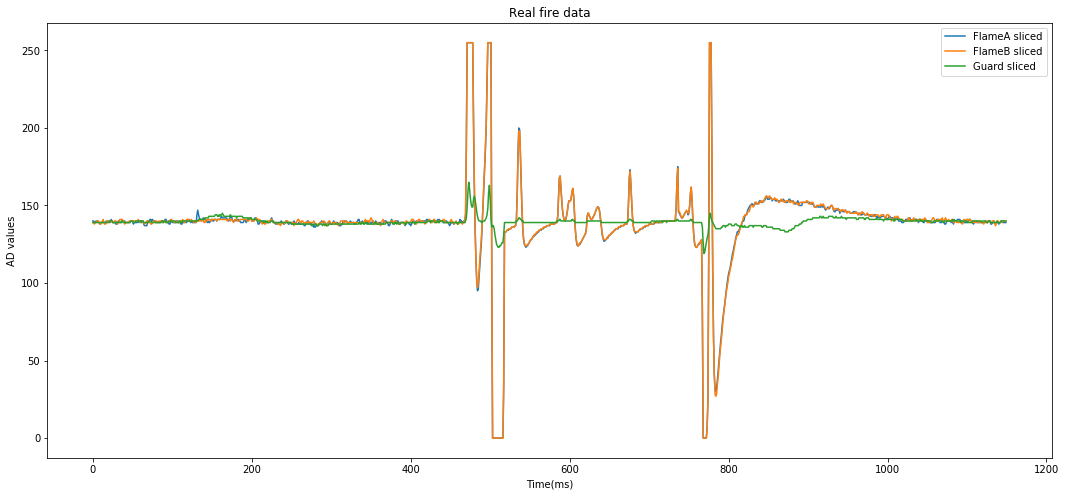
\includegraphics[width=\columnwidth]{pictures/01-real-fire-data.png}
 \caption{Closely overlapping Flame A and Flame B fire data}
 \label{fig:sample}
\end{figure}

\subsection{Noise data}

We plotted the same section of our noise data and found that Flame A and Flame B did not overlapped, in fact in parts they were going in opposite directions (antiphase), finding that this could become an engineered feature.

\begin{figure}[tb]
 \centering % avoid the use of \begin{center}...\end{center} and use \centering instead (more compact)
 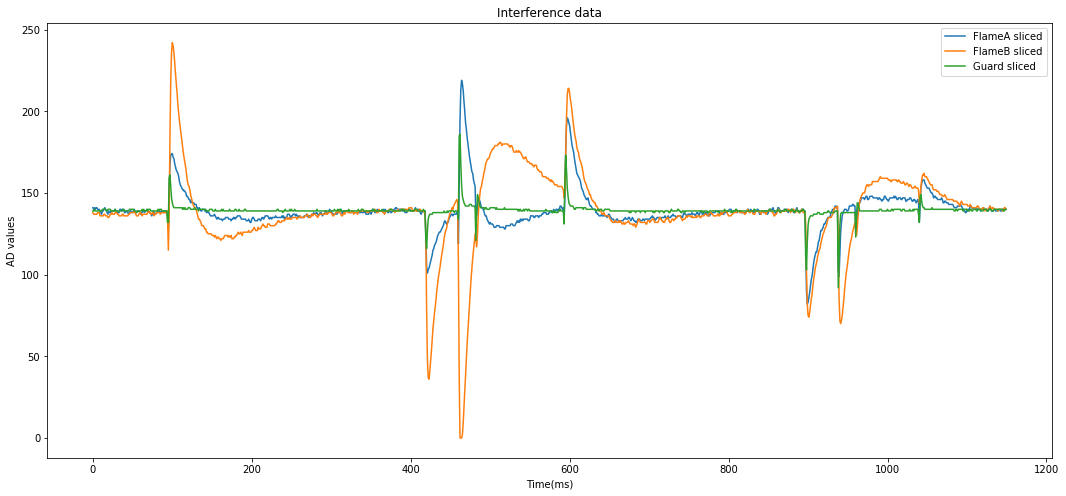
\includegraphics[width=\columnwidth]{pictures/02-interference-data.png}
 \caption{Interference plot, Flame A and Flame B with little or no overlap}
 \label{fig:sample}
\end{figure}

\subsection{Data normalisation}

We normalised our data, initially using a per-attribute minimum and maximum values:

$$ z{_i}=\frac{x{_i}-min(x)}{max(x)-min(x)} ,max(x)-min(x) \neq 0 $$

And found that this approach distorted our plot.

\begin{figure}[tb]
 \centering % avoid the use of \begin{center}...\end{center} and use \centering instead (more compact)
 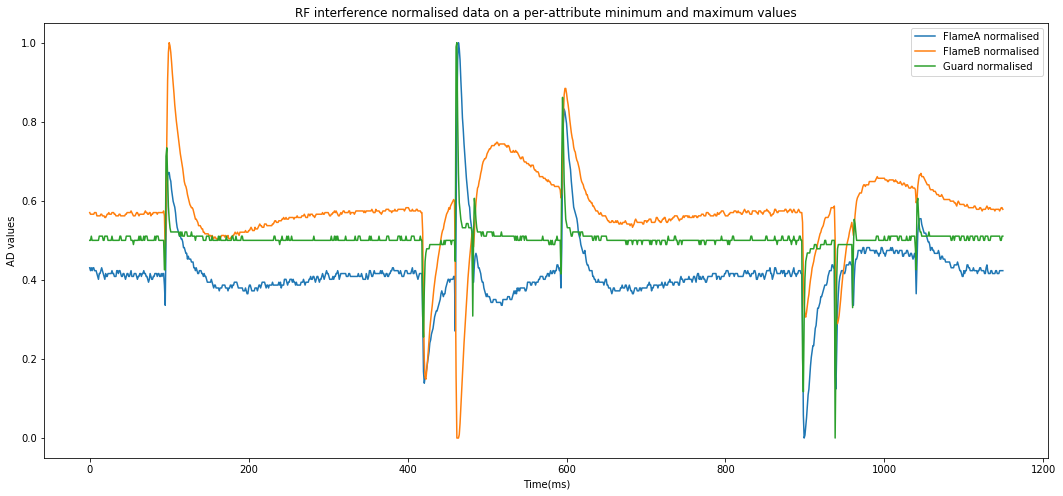
\includegraphics[width=\columnwidth]{pictures/03-interference-data-normalised-per-attribute-min-max.png}
 \caption{Normalised plot with distortion, per attribute minimum and maximum values}
 \label{fig:sample}
\end{figure}

So we modified the normalisation algorithm using minimum and maximum values across all attributes as they are scaled to same values (0-255)

$$ z{_i}=\frac{x{_i}-min}{max-min} , max-min \neq 0 $$

\subsection{Distance function}

Once our data was normalised, we created a distance function expecting that this would provide a measure to distinguish noise from signal. This approach was based on the degree of overlapping presented by Flame A and Flame B signals for fire data and inteference data. we obtained the distance value by the absolute difference of Flame A and Flame B

$$ Fd = |Nfa - Nfb| $$

With this engineered attribute we plotted both features to find that interference data presented, as expected, greater distances and fire data.

\begin{figure}[tb]
 \centering % avoid the use of \begin{center}...\end{center} and use \centering instead (more compact)
 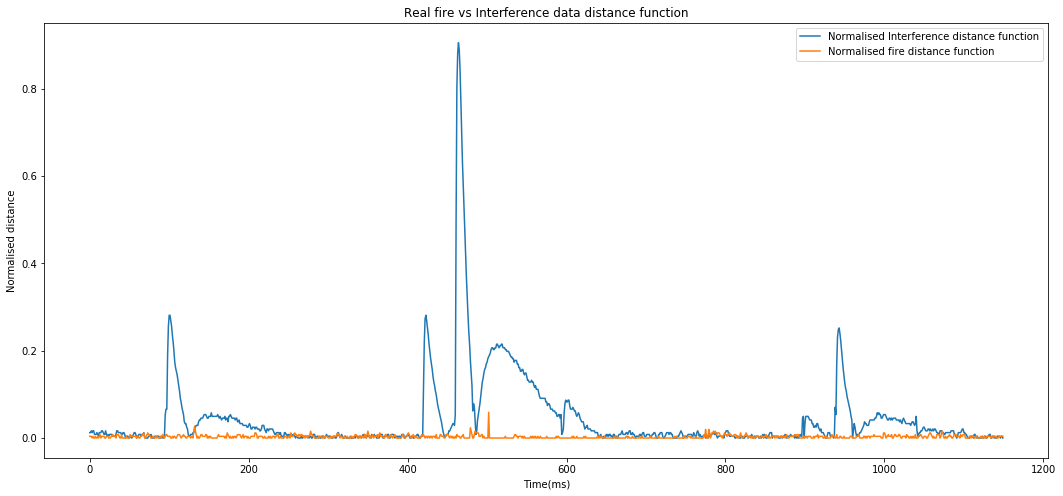
\includegraphics[width=\columnwidth]{pictures/06-fire-interference-distance-function.png}
 \caption{Fire and interference distance function}
 \label{fig:sample}
\end{figure}

\subsection{Linear regression}

Since the distance function showed how closely the signals of Flame A and Flame B were match, we figured it would be a good idea to plot our data plus a line of best fit, to confirm our findings using a well established approach.  
The interference data proved to have a weak positive correlation, while the fire data proved to have a strong positive correlation.

\begin{figure}[tb]
 \centering % avoid the use of \begin{center}...\end{center} and use \centering instead (more compact)
 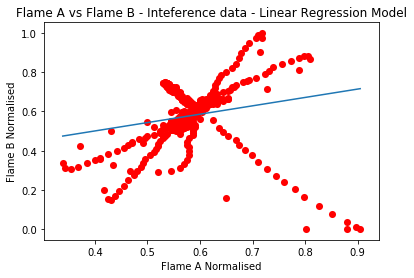
\includegraphics[width=\columnwidth]{pictures/07-interference-linear-regression.png}
 \caption{Interference linear regression - weak positive correlation}
 \label{fig:sample}
\end{figure}

\begin{figure}[tb]
 \centering % avoid the use of \begin{center}...\end{center} and use \centering instead (more compact)
 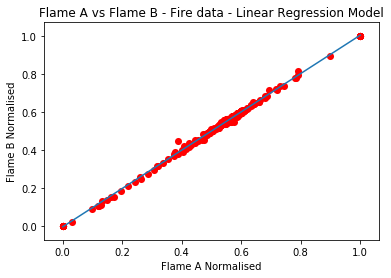
\includegraphics[width=\columnwidth]{pictures/08-fire-linear-regression.png}
 \caption{Fire data linear regression - strong positive correlation}
 \label{fig:sample}
\end{figure}

\subsection{Antiphase}

Our second and last engineered function was the antiphase flag, that is true whenever Flame A and Flame B signals are moving in opposite directions. This can be determined by dividing the deltas and verifying the sign, if it is found to be negative, the signals are in antiphase.

$$  A \Rightarrow \frac{\Delta Fa}{\Delta Fb}<0$$
where
$$ \Delta Fa = Fa{_i}-Fa{_{i-1}}, \Delta Fb = Fb{_i}-Fb{_{i-1}}, \forall i > 1 $$

With the antiphase attribute we were able to overlay this new attribute with the original plots. This showed us that interference data showed antiphase signals throughout the plot while fire data showed no antiphase in the fire signal section, suggesting that Flame A and Flame B were tightly overlapped.

We did notice however that the antiphase flag was not set throughout signals that visually appeared to be moving in opposite directions, this suggested there is further scope for improvement in the antiphase algorithm, perhaps using a window as in an interval of values, instead of discreet values, and this could be carried out in future works.

\begin{figure}[tb]
 \centering % avoid the use of \begin{center}...\end{center} and use \centering instead (more compact)
 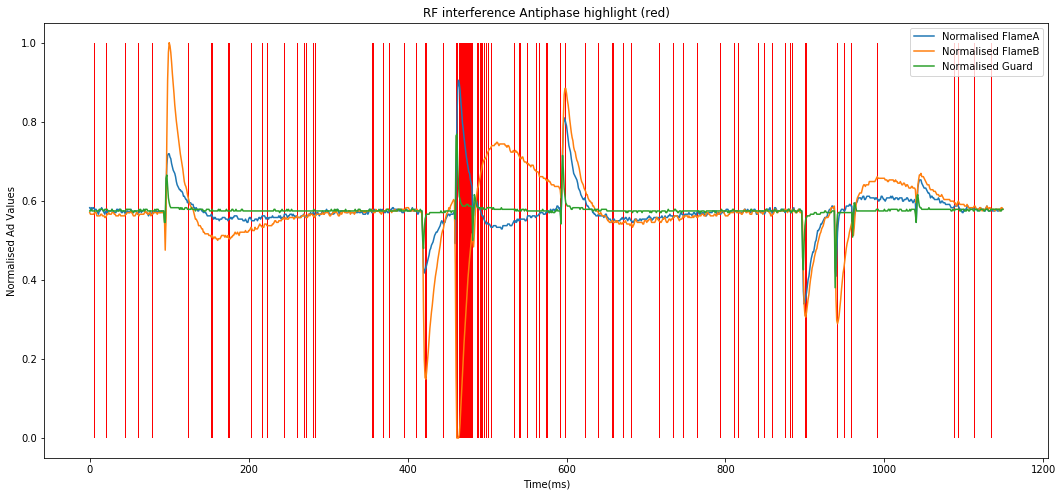
\includegraphics[width=\columnwidth]{pictures/09-interference-antiphase.png}
 \caption{Interference antiphase highlight (red)}
 \label{fig:sample}
\end{figure}

\begin{figure}[tb]
 \centering % avoid the use of \begin{center}...\end{center} and use \centering instead (more compact)
 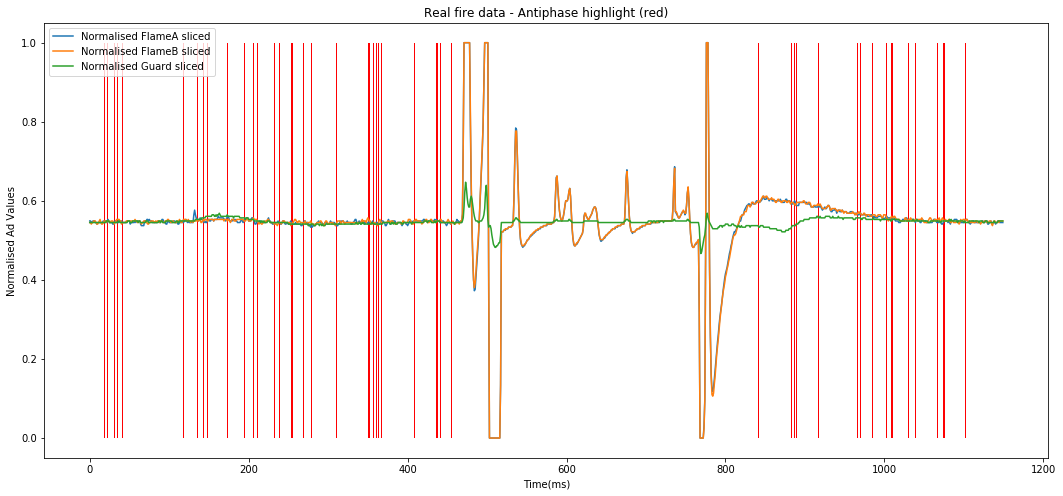
\includegraphics[width=\columnwidth]{pictures/10-fire-antiphase.png}
 \caption{Fire antiphase highlight (red)}
 \label{fig:sample}
\end{figure}


Between our distance function and antiphase function, we believe there is enough data to safely distinguish signal and noise which would have commercial applications in ensuring equipment would pass security integrity level approval tests. 

In addition to our engineer attributes, we also attempted fast fourier transforms which did not provide clear pointers, in this instance, as to the usefulness of the approach.

We first transformed noisy data obtaining a frequency plot, then replotted with data smoothed using the Savistzky-Golay filter, and found the frequency showed more regularity, by the increased number of zero crossing observed.

We then plotted the data with no filter applied, which showed a slightly noisier signal as expected, then the same data with a filter applied with is slightly smoother.

\begin{figure}[tb]
 \centering % avoid the use of \begin{center}...\end{center} and use \centering instead (more compact)
 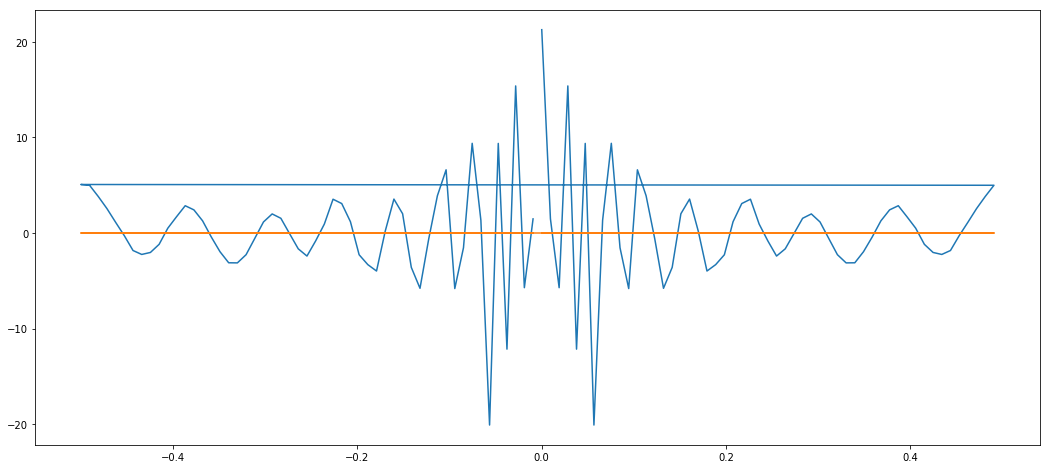
\includegraphics[width=\columnwidth]{pictures/15-inteference-slice-smoothed-fft.png}
 \caption{Interference slice smoothed fast fourier transform}
 \label{fig:sample}
\end{figure}


%% if specified like this the section will be committed in review mode

%%%%%%%%%%%%%%%%%%%%%%%%%%%%%%%%%%%%%%%%%%%%%%%%%%%%%%%%%%%%%%%%
%%%%%%%%%%%%%%%%%%%%%% ACKNOWLEDGEMENTS %%%%%%%%%%%%%%%%%%%%%%%%
%%%%%%%%%%%%%%%%%%%%%%%%%%%%%%%%%%%%%%%%%%%%%%%%%%%%%%%%%%%%%%%%

\acknowledgments{
We wish to thank Abi, Alex, Cagatay, Mirela and Phong for their enthusiasm, guidance and support, and Aidan Slingsby for the \LaTeX/bib\TeX\ template  used to format this text.}

%\bibliographystyle{abbrv}
\bibliographystyle{abbrv-doi}
%\bibliographystyle{abbrv-doi-narrow}
%\bibliographystyle{abbrv-doi-hyperref}
%\bibliographystyle{abbrv-doi-hyperref-narrow}

\bibliography{INM430-final-report}
\end{document}

